\documentclass[11pt, oneside]{article}
\usepackage[margin=1in,letterpaper]{geometry}
\usepackage{times}
\usepackage{graphicx}
\usepackage{amssymb,amsmath}
\usepackage{array}
\usepackage{longtable}
\usepackage{color}
\usepackage[T1]{fontenc}
\usepackage{sectsty}
\usepackage{tikz}
\usepackage{pgfplots}
\pgfplotsset{compat=1.17}
\sectionfont{\fontsize{12}{12}\selectfont}
\subsectionfont{\fontsize{11}{11}\selectfont}
\subsubsectionfont{\normalsize\itshape\mdseries}

\renewcommand\labelitemi{{\boldmath$\cdot$}}

%%%%%%%%%%%%%%%%%%%%%%%%%%%%%%%%%%%%%
% Notation: vectors are bold (handwritten: underlined); unit vectors are \hat{\mathbf{x}}, etc.
% Following the master table (D2, D12), phasors carry a tilde: E(x,y,z,t) = Re[E~(x,y,z) e^{jwt}].
% Per the master table: phase velocity u_p (D15), lowercase wavenumber k (D14), Poynting vector in script S (D10),
% amplitudes E^i, E^r, E^t without subscript 0 (D27), transmissivity blackboard T (D19);
% the handwriting uses v_p, capital K, plain S, E_0^i (and E_{h0}^i, E_{0z}^i), and T.
% The handwriting writes the fields with e^{j(k.r - wt)}; converted to the course convention e^{jwt},
% i.e., phasors with e^{-j k.r} (as on the handwritten page with the H-polarized fields, which uses e^{-gamma(...)}).
% The phase of eta is phi_eta, as handwritten here; adopted course-wide (Lectures 2 and 4 updated; master table D29),
% so the handwritten "note change of variable from previous lectures" no longer applies. The complex angle of refraction
% is written with a tilde, tilde(theta)_t (D32); the critical angle is theta_c (D35; handwritten theta_*).
%%%%%%%%%%%%%%%%%%%%%%%%%%%%%%%%%%%%%

\title{12.421/12.621 Lecture 5: Reflection and Transmission of EM Waves at Oblique Incidence}
\author{Brent Minchew}
\date{}

\begin{document}
\maketitle

\noindent\textbf{Topics covered}
\begin{itemize}
	\item Reflection and transmission at oblique incidence
\end{itemize}

%%%%%%%%%%%%%%%%%%%%%%%%%%%%%%%%%%%%%
\section{EM boundary conditions (review)}

% NOTE: added "(Lecture 4)" and "in lossless media" (the BCs on eps' eps_0 E hold as written for lossless media;
% Lecture 4 summary, same scope). The handwritten underlined vectors are written bold.
The EM boundary conditions (BCs) for zero charge and zero current at the interface, in lossless media (Lecture 4), with $\hat{\mathbf{a}}$ the unit normal to the interface, are:
\begin{enumerate}
	\item $\varepsilon_1'E_1^\perp = \varepsilon_2'E_2^\perp$ \quad or \quad $\hat{\mathbf{a}}\cdot\left(\varepsilon_1'\mathbf{E}_1 - \varepsilon_2'\mathbf{E}_2\right) = 0$
	\begin{itemize}
		\item[] $\rightarrow$ the normal component of $\varepsilon'\mathbf{E}$ is continuous;
	\end{itemize}
	\item $\mu_1H_1^\perp = \mu_2H_2^\perp$ \quad or \quad $\hat{\mathbf{a}}\cdot\left(\mu_1\mathbf{H}_1 - \mu_2\mathbf{H}_2\right) = 0$
	\begin{itemize}
		\item[] $\rightarrow$ the normal component of $\mu\mathbf{H}$ is continuous;
	\end{itemize}
	\item $\mathbf{E}_1^\parallel = \mathbf{E}_2^\parallel$ \quad or \quad $\hat{\mathbf{a}}\times\left(\mathbf{E}_1 - \mathbf{E}_2\right) = \mathbf{0}$
	\begin{itemize}
		\item[] $\rightarrow$ the tangential component of $\mathbf{E}$ is continuous;
	\end{itemize}
	\item $\mathbf{H}_1^\parallel = \mathbf{H}_2^\parallel$ \quad or \quad $\hat{\mathbf{a}}\times\left(\mathbf{H}_1 - \mathbf{H}_2\right) = \mathbf{0}$
	\begin{itemize}
		\item[] $\rightarrow$ the tangential component of $\mathbf{H}$ is continuous.
	\end{itemize}
\end{enumerate}

%%%%%%%%%%%%%%%%%%%%%%%%%%%%%%%%%%%%%
\section{Reflection and transmission at oblique incidence: geometric optics}

Let's start with the basics: ``geometric optics'' (Figure~\ref{f:geometry}).

\begin{figure}[h]
	\centering
	% Elements follow the handwritten sketch: z and x axes, medium 1 (top) and medium 2 (bottom) labels,
	% wavenumber vectors k_i (arrow pointing into the origin), k_r, k_t, and angles theta_i, theta_r, theta_t
	% measured from the normal. Illustrative angles: theta_i = 30 deg, theta_t = 12 deg.
	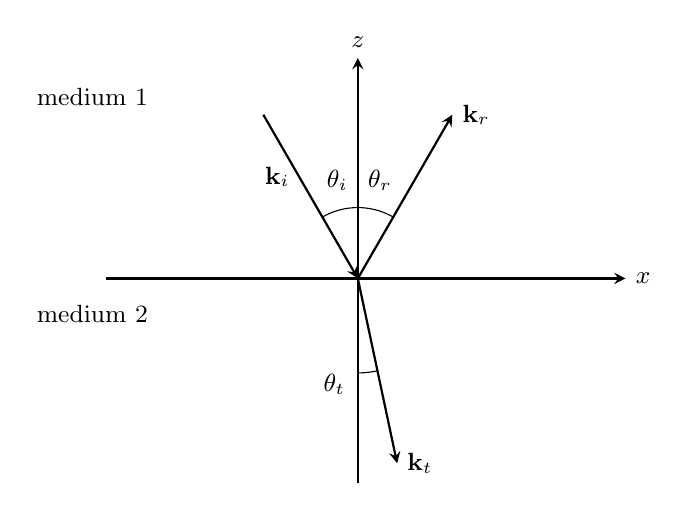
\begin{tikzpicture}[>=stealth, font=\small]
		\def\ti{30}\def\tt{12}\def\L{2.4}
		\draw[->, thick] (-3.2,0) -- (3.4,0) node[right] {$x$};
		\draw[->, thick] (0,-2.6) -- (0,2.8) node[above] {$z$};
		\node[anchor=west] at (-4.2,2.3) {medium 1};
		\node[anchor=west] at (-4.2,-0.45) {medium 2};
		% incident (arrow into the origin), reflected, transmitted
		\draw[->, thick] ({-\L*sin(\ti)},{\L*cos(\ti)}) -- (0,0);
		\node[left] at ({-0.62*\L*sin(\ti)},{0.62*\L*cos(\ti)}) {$\mathbf{k}_i$};
		\draw[->, thick] (0,0) -- ({\L*sin(\ti)},{\L*cos(\ti)}) node[right] {$\mathbf{k}_r$};
		\draw[->, thick] (0,0) -- ({\L*sin(\tt)},{-\L*cos(\tt)}) node[right] {$\mathbf{k}_t$};
		% angles
		\draw (0,0.9) arc (90:{90+\ti}:0.9);
		\node at ({-0.26},1.25) {$\theta_i$};
		\draw (0,0.9) arc (90:{90-\ti}:0.9);
		\node at ({0.28},1.25) {$\theta_r$};
		\draw (0,-1.2) arc (270:{270+\tt}:1.2);
		\node at ({-0.3},-1.35) {$\theta_t$};
	\end{tikzpicture}
	\caption{Geometry of reflection and transmission at oblique incidence on the planar interface ($z = 0$) between medium 1 and medium 2. $\mathbf{k}_i$ is the wavenumber vector of the incident wave (and similarly $\mathbf{k}_r$ and $\mathbf{k}_t$ for the reflected and transmitted waves).}
	\label{f:geometry}
\end{figure}

\subsection{Fields for a uniform plane wave}

% NOTE: handwritten writes E^i(r,t) = E_0^i e^{j(k_i . r - w t)} (physics convention e^{-jwt}) with capital K and a
% vector amplitude E_0^i; converted to the course convention e^{jwt} (master table, Conventions), with phasors
% carrying a tilde (D12) and the amplitude written as the phasor at the origin, E~^i(0), to avoid the subscript 0 (D27).
% Both forms describe the same waves. Added "(Lecture 2)" for the relation H = (1/eta) k x E.
With position vector $\mathbf{r}$, the fields of the incident, reflected, and transmitted uniform plane waves are, in terms of phasors [$\mathbf{E}^i(\mathbf{r},t) = \mathrm{Re}\{\tilde{\mathbf{E}}^i(\mathbf{r})\,e^{j\omega t}\}$, etc.],
\begin{align}
	\text{incident:} \quad &
	\tilde{\mathbf{E}}^i(\mathbf{r}) = \tilde{\mathbf{E}}^i(\mathbf{0})\,e^{-j\mathbf{k}_i\cdot\mathbf{r}}, &
	\tilde{\mathbf{H}}^i(\mathbf{r}) &= \frac{1}{\eta_1}\left(\hat{\mathbf{k}}_i\times\tilde{\mathbf{E}}^i(\mathbf{r})\right), \label{e:field_i}\\
	\text{reflected:} \quad &
	\tilde{\mathbf{E}}^r(\mathbf{r}) = \tilde{\mathbf{E}}^r(\mathbf{0})\,e^{-j\mathbf{k}_r\cdot\mathbf{r}}, &
	\tilde{\mathbf{H}}^r(\mathbf{r}) &= \frac{1}{\eta_1}\left(\hat{\mathbf{k}}_r\times\tilde{\mathbf{E}}^r(\mathbf{r})\right), \label{e:field_r}\\
	\text{transmitted:} \quad &
	\tilde{\mathbf{E}}^t(\mathbf{r}) = \tilde{\mathbf{E}}^t(\mathbf{0})\,e^{-j\mathbf{k}_t\cdot\mathbf{r}}, &
	\tilde{\mathbf{H}}^t(\mathbf{r}) &= \frac{1}{\eta_2}\left(\hat{\mathbf{k}}_t\times\tilde{\mathbf{E}}^t(\mathbf{r})\right), \label{e:field_t}
\end{align}
where $\hat{\mathbf{k}}_i = \mathbf{k}_i/k_i$, etc., are the propagation unit vectors (Lecture 2).

\begin{itemize}
	\item Recall that $\omega$ is the same everywhere and for all time and is set by the source.
	\item[] $\Rightarrow$ the dispersion relation gives
	\begin{equation}
		\omega = k_iu_{p1} = k_ru_{p1} = k_tu_{p2}
	\end{equation}
	% NOTE: the n'-based relation is exact for lossless media (U&L 2014, Sec. 2-7 assumes lossless media, p. 54);
	% for oblique incidence onto a lossy medium the transmitted wave is not a uniform plane wave and the
	% phase-matching condition is gamma_1 sin theta_i = gamma_2 sin theta_t (Section s:lossy; U&L Eq. 2.113).
	% E.g., eps_1 = 1, eps_2 = 3 - j3, theta_i = 60 deg: sin theta_t = sin theta_i / n_2' gives 27.1 deg vs. the
	% physical 26.6 deg (python3). Added "(lossless media; see Section s:lossy for lossy media)".
	\begin{equation}
		\label{e:k_ratio}
		\Rightarrow\quad
		\boxed{k_i = k_r = \frac{u_{p2}}{u_{p1}}\,k_t = \frac{\mathrm{Re}\left(\sqrt{\varepsilon_1}\right)}{\mathrm{Re}\left(\sqrt{\varepsilon_2}\right)}\,k_t = \frac{n_1'}{n_2'}\,k_t}
	\end{equation}
	(lossless media; see Section~\ref{s:lossy} for lossy media).
	\item The total $\mathbf{E}$ and $\mathbf{H}$ fields in medium 1 are related to those in medium 2 through the BCs, which have the generic structure
	% NOTE: handwritten labels the coefficients B_i^i, B_r^r, B_t^t; the repeated label is written once (B^i, B^r, B^t).
	\begin{equation}
		\label{e:generic}
		B^i\,e^{j(\omega t - \mathbf{k}_i\cdot\mathbf{r})} + B^r\,e^{j(\omega t - \mathbf{k}_r\cdot\mathbf{r})} = B^t\,e^{j(\omega t - \mathbf{k}_t\cdot\mathbf{r})}.
	\end{equation}
	Don't worry about the $B$ coefficients for now; just note that the only space and time dependence is in the exponents.
\end{itemize}

\subsection{Matching the exponents at the interface}

\begin{itemize}
	\item The BCs must hold everywhere on the $xy$ plane at the interface $z = 0$ for all times.
	\item[] $\Rightarrow$ the exponential factors in Eq.~\eqref{e:generic} must be equal at $z = 0$:
	\begin{itemize}
		\item the time factors are already equal because $\omega = $ const;
		\item the spatial components give
		\begin{equation}
			\mathbf{k}_i\cdot\mathbf{r} = \mathbf{k}_r\cdot\mathbf{r} = \mathbf{k}_t\cdot\mathbf{r} \qquad \text{at } z = 0.
		\end{equation}
		Expanding,
		\begin{equation}
			xk_{ix} + yk_{iy} = xk_{rx} + yk_{ry} = xk_{tx} + yk_{ty}
		\end{equation}
		\underline{\underline{for all $x$ and $y$}} $\Rightarrow$ this only holds if the components are separately equal:
		\begin{itemize}
			\item[$\hookrightarrow$] for $x = 0$: \quad $k_{iy} = k_{ry} = k_{ty}$;
			\item[$\hookrightarrow$] for $y = 0$: \quad $k_{ix} = k_{rx} = k_{tx}$.
		\end{itemize}
	\end{itemize}
	\item We are free to choose our coordinate system; for convenience, let's define $\mathbf{k}_i$ to lie in the $x$--$z$ plane
	\begin{equation}
		\Rightarrow\quad k_{iy} = k_{ry} = k_{ty} = 0,
	\end{equation}
	and the only non-zero components of the wavenumber vectors lie in the $x$--$z$ plane for the incident, reflected, and transmitted waves.
\end{itemize}

\subsection{The three laws of geometric optics}

From the above, we get

\begin{center}
\fbox{\begin{minipage}{0.9\linewidth}
	\textbf{1st law of geometric optics:} The incident, reflected, and transmitted wave vectors (rays) form a plane called the \emph{plane of incidence}, which also includes the normal to the surface (in our case $\hat{\mathbf{z}}$).
\end{minipage}}
\end{center}

Now, given that $k_{ix} = k_{rx} = k_{tx}$,
\begin{equation}
	\label{e:phase_match}
	k_i\sin\theta_i = k_r\sin\theta_r = k_t\sin\theta_t,
\end{equation}
where, all measured with respect to the normal,
\begin{itemize}
	\item $\theta_i \equiv$ angle of incidence;
	\item $\theta_r \equiv$ angle of reflection;
	\item $\theta_t \equiv$ angle of refraction (or transmission).
\end{itemize}
From the dispersion relation, we have $k_i = k_r$, so
\begin{equation}
	\boxed{\theta_i = \theta_r \equiv \theta_1}
\end{equation}

\begin{center}
\fbox{\begin{minipage}{0.9\linewidth}
	\textbf{2nd law of geometric optics}, commonly called the \emph{law of reflection}: angle of incidence $\theta_i$ = angle of reflection $\theta_r$.
\end{minipage}}
\end{center}

And from the dispersion relation, we have [Eq.~\eqref{e:k_ratio}]
\begin{equation}
	k_i = k_r = k_1 = \frac{u_{p2}}{u_{p1}}\,k_t = \frac{\mathrm{Re}\left(\sqrt{\varepsilon_1}\right)}{\mathrm{Re}\left(\sqrt{\varepsilon_2}\right)}\,k_t = \frac{n_1'}{n_2'}\,k_t.
\end{equation}

% NOTE: added "(lossless media)" for the reason given at Eq. (e:k_ratio); cf. U&L 2014, Eqs. 2.95, 2.97.
\begin{center}
\fbox{\begin{minipage}{0.9\linewidth}
	\textbf{3rd law of geometric optics}, a.k.a.\ the \emph{law of refraction} or \emph{Snell's law} (lossless media):
	\begin{equation}
		\label{e:snell}
		\frac{\sin\theta_t}{\sin\theta_i} = \frac{u_{p2}}{u_{p1}} = \frac{n_1'}{n_2'} = \frac{\mathrm{Re}\left(\sqrt{\varepsilon_1}\right)}{\mathrm{Re}\left(\sqrt{\varepsilon_2}\right)}
	\end{equation}
\end{minipage}}
\end{center}

\begin{itemize}
	\item Note that up to this point, we did \underline{not} invoke any EM principles to derive the three laws of geometric optics.
	\item[] $\Rightarrow$ These laws are valid for all wave types (water, sound, seismic, etc.), and many of you will have seen them before.
\end{itemize}

\subsection{Implications of Snell's law}

Before moving on to EM waves, let's quickly consider the implications of Snell's law. Let's keep it simple and consider lossless media (Figure~\ref{f:snell}).

\begin{figure}[h]
	\centering
	% Elements follow the three handwritten sketches: z and x axes, incident ray with its arrow at the origin,
	% reflected and transmitted rays with arrowheads, angle arcs theta_i, theta_i, theta_t (from -z), eps_1', eps_2'
	% labels in (a), and the right-angle mark in (c). Illustrative angles: theta_i = 30 deg; theta_t = 12 deg (a),
	% 60 deg (b), 90 deg (c).
	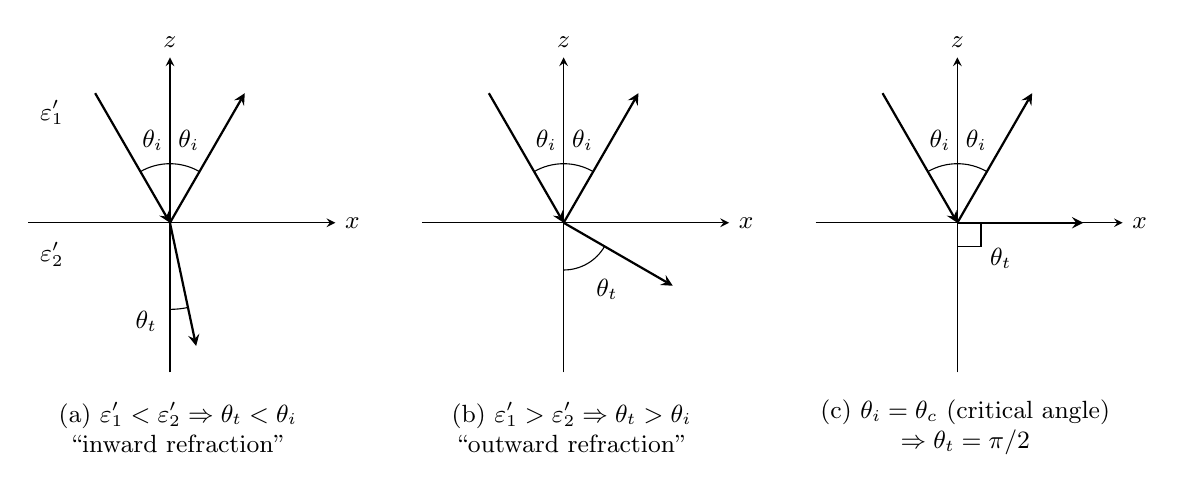
\begin{tikzpicture}[>=stealth, font=\small]
		\def\ti{30}\def\L{1.9}
		\foreach \xs/\tt/\lab in {0/12/a, 5.0/60/b, 10.0/90/c} {
			\begin{scope}[xshift=\xs cm]
				\draw[->] (-1.8,0) -- (2.1,0) node[right] {$x$};
				\draw[->] (0,-1.9) -- (0,2.1) node[above] {$z$};
				\draw[->, thick] ({-\L*sin(\ti)},{\L*cos(\ti)}) -- (0,0);
				\draw[->, thick] (0,0) -- ({\L*sin(\ti)},{\L*cos(\ti)});
				\draw (0,0.75) arc (90:{90+\ti}:0.75);
				\draw (0,0.75) arc (90:{90-\ti}:0.75);
				\node at (-0.22,1.05) {$\theta_i$};
				\node at (0.24,1.05) {$\theta_i$};
				\draw[->, thick] (0,0) -- ({1.6*sin(\tt)},{-1.6*cos(\tt)});
			\end{scope}
		}
		% (a) inward refraction
		\draw (0,-1.1) arc (270:282:1.1);
		\node at (-0.3,-1.25) {$\theta_t$};
		\node at (-1.5,1.4) {$\varepsilon_1'$};
		\node at (-1.5,-0.4) {$\varepsilon_2'$};
		\node[align=center] at (0.1,-2.6) {(a) $\varepsilon_1' < \varepsilon_2' \Rightarrow \theta_t < \theta_i$\\``inward refraction''};
		% (b) outward refraction
		\draw (5.0,-0.6) arc (270:330:0.6);
		\node at (5.55,-0.85) {$\theta_t$};
		\node[align=center] at (5.1,-2.6) {(b) $\varepsilon_1' > \varepsilon_2' \Rightarrow \theta_t > \theta_i$\\``outward refraction''};
		% (c) critical angle: right-angle mark between -z and the transmitted ray along the boundary
		\draw (10.0,-0.3) -- (10.3,-0.3) -- (10.3,0);
		\node at (10.55,-0.45) {$\theta_t$};
		\node[align=center] at (10.1,-2.6) {(c) $\theta_i = \theta_c$ (critical angle)\\$\Rightarrow \theta_t = \pi/2$};
	\end{tikzpicture}
	\caption{Implications of Snell's law for lossless media: (a) inward refraction ($\varepsilon_1' < \varepsilon_2'$); (b) outward refraction ($\varepsilon_1' > \varepsilon_2'$); (c) incidence at the critical angle $\theta_c$, where the refracted wave travels along the boundary.}
	\label{f:snell}
\end{figure}

\begin{itemize}
	\item $\varepsilon_1' < \varepsilon_2'$ $\Rightarrow$ $\theta_t < \theta_i$: ``inward refraction'' (Figure~\ref{f:snell}a).
	\item $\varepsilon_1' > \varepsilon_2'$ $\Rightarrow$ $\theta_t > \theta_i$: ``outward refraction'' (Figure~\ref{f:snell}b).
	% NOTE: the handwritten critical-angle symbol theta_* is written theta_c, as in U&L 2014, Eq. 2.98 (master table D35).
	\item \emph{Critical angle:} $\theta_i = \theta_c \rightarrow \theta_t = \pi/2$ (Figure~\ref{f:snell}c). To find $\theta_c$, apply Snell's law:
	\begin{equation}
		\sin\theta_c = \frac{n_2'}{n_1'}\sin\theta_t\bigg|_{\theta_t = \pi/2} = \frac{n_2'}{n_1'}
		\quad\Rightarrow\quad
		\theta_c = \sin^{-1}\left(\frac{\mathrm{Re}\left(\sqrt{\varepsilon_2}\right)}{\mathrm{Re}\left(\sqrt{\varepsilon_1}\right)}\right).
	\end{equation}
	\begin{itemize}
		\item When $\theta_i = \theta_c$, the refracted wave travels along the boundary.
		\item When $\theta_i > \theta_c$: total reflection (only possible when $n_1' > n_2'$).
		\begin{itemize}
			\item[$\hookrightarrow$] gives diamonds sparkle.
		\end{itemize}
	\end{itemize}
\end{itemize}

%%%%%%%%%%%%%%%%%%%%%%%%%%%%%%%%%%%%%
\section{Reflection and transmission of EM waves at oblique incidence}

Now that we have an okay grasp of the exponential terms, let's return to EM waves.

\subsection{Applying the boundary conditions}

% NOTE: handwritten writes the amplitudes as E_{0z}^i, H_{0x}^i, etc.; written as the components of the phasors at the
% origin, E~^i_z = z . E~^i(0), etc. (D12, D27). Because the exponential factors are equal on z = 0, the BCs apply
% to these amplitudes directly. Added this sentence as a minimal clarification.
Applying the BCs discussed before to the components of the field phasors at the origin (the exponential factors are equal everywhere on $z = 0$):
\begin{enumerate}
	\item Gauss's law:
	\begin{equation}
		\label{e:bc_gauss}
		\varepsilon_1'\left(\tilde{E}^i_z + \tilde{E}^r_z\right) = \varepsilon_2'\tilde{E}^t_z;
	\end{equation}
	\item Gauss's law for magnetism:
	\begin{equation}
		\label{e:bc_gaussm}
		\mu_1\left(\tilde{H}^i_z + \tilde{H}^r_z\right) = \mu_2\tilde{H}^t_z;
	\end{equation}
	\item Faraday's law:
	\begin{equation}
		\label{e:bc_faraday}
		\tilde{E}^i_x + \tilde{E}^r_x = \tilde{E}^t_x, \qquad \tilde{E}^i_y + \tilde{E}^r_y = \tilde{E}^t_y;
	\end{equation}
	\item Amp\`ere's law:
	\begin{equation}
		\label{e:bc_ampere}
		\tilde{H}^i_x + \tilde{H}^r_x = \tilde{H}^t_x, \qquad \tilde{H}^i_y + \tilde{H}^r_y = \tilde{H}^t_y.
	\end{equation}
\end{enumerate}

\subsection{Polarization definitions}

Now we need to get organized by defining polarizations.
\begin{itemize}
	\item What's a good reference for polarization? The plane of incidence (see the 1st law of geometric optics).
	\item[] $\Rightarrow$ two commonly defined polarizations (Figure~\ref{f:pol}):
	\begin{enumerate}
		\item \emph{perpendicular} or \emph{horizontal} $\rightarrow$ the $\mathbf{E}$ field is normal to the plane of incidence;
		\item \emph{parallel} or \emph{vertical} $\rightarrow$ the $\mathbf{H}$ field is normal to the plane of incidence (so named because the $\mathbf{E}$ field lies in the plane of incidence and usually has a vertical component).
	\end{enumerate}
\end{itemize}

\begin{figure}[h]
	\centering
	% Elements follow the handwritten sketches: z and x axes; eps_1, eps_2 labels in (a); incident, reflected, and
	% transmitted rays; at each wave, the field normal to the plane of incidence (circle), the in-plane field arrow,
	% and the propagation unit vector; angle arcs theta_i, theta_i, theta_t (from -z).
	% Illustrative angles: theta_i = 35 deg, theta_t = 18 deg.
	% NOTE: the handwritten (a) labels the transmitted propagation vector "k_h"; corrected to k_t (cf. panel b).
	% NOTE: in the handwritten (b), the reflected wave has H_v^r into the page and E_v^r pointing down and to the right
	% (as in U&L 2014, Fig. 2-16b, p. 56, and the V-polarized E^r, H^r rows of Table 2-4, p. 58). With those
	% reference directions, the BCs give E_v^r/E_v^i = (eta_1 cos th_i - eta_2 cos th_t)/(eta_1 cos th_i + eta_2 cos th_t),
	% the negative of rho_v in Eq. (e:rho_v) (U&L Eq. 2.102a and Table 2-5, p. 61); tau_v is unchanged, since E^t keeps its
	% reference direction (derived; checked in python3 by the conversion agent, the checker, and in screening). Reversed E_v^r (now up and to the left) and H_v^r (now out of
	% the page) so that the sketch is consistent with rho_v and tau_v below and with rho_v = rho_h = rho at normal
	% incidence (Lecture 4). All other elements are as drawn. (U&L Table 2-4 also has eta_1 where eta_2 belongs in H_v^t.)
	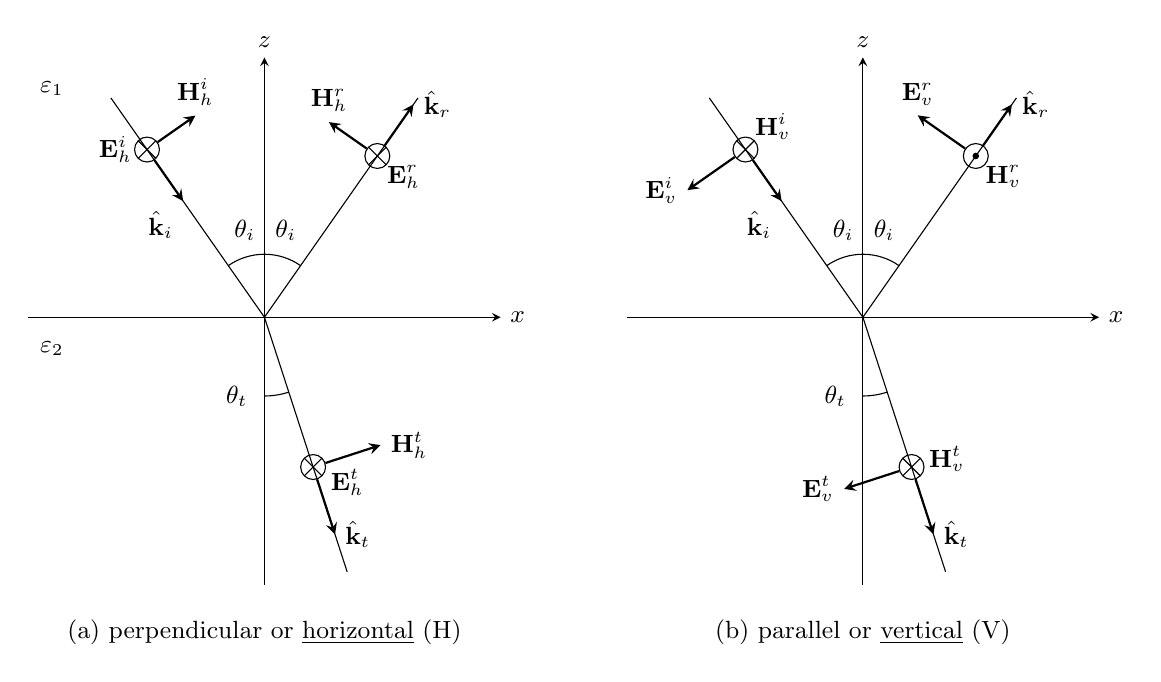
\begin{tikzpicture}[>=stealth, font=\small,
		otimes/.style={circle, draw, inner sep=0pt, minimum size=9pt, path picture={
			\draw (path picture bounding box.north west) -- (path picture bounding box.south east)
				(path picture bounding box.south west) -- (path picture bounding box.north east);}},
		odot/.style={circle, draw, inner sep=0pt, minimum size=9pt, path picture={
			\fill (path picture bounding box.center) circle (1.2pt);}}]
		\def\ti{35}\def\tt{18}
		% ---------------- (a) horizontal polarization ----------------
		\begin{scope}
			\draw[->] (-3.0,0) -- (3.0,0) node[right] {$x$};
			\draw[->] (0,-3.4) -- (0,3.3) node[above] {$z$};
			\node at (-2.7,2.9) {$\varepsilon_1$};
			\node at (-2.7,-0.4) {$\varepsilon_2$};
			\draw[thin] ({-3.4*sin(\ti)},{3.4*cos(\ti)}) -- (0,0) -- ({3.4*sin(\ti)},{3.4*cos(\ti)});
			\draw[thin] (0,0) -- ({3.4*sin(\tt)},{-3.4*cos(\tt)});
			\draw (0,0.8) arc (90:{90+\ti}:0.8);
			\draw (0,0.8) arc (90:{90-\ti}:0.8);
			\node at (-0.25,1.1) {$\theta_i$};
			\node at (0.27,1.1) {$\theta_i$};
			\draw (0,-1.0) arc (270:{270+\tt}:1.0);
			\node at (-0.35,-1.0) {$\theta_t$};
			% incident
			\coordinate (Ci) at ({-2.6*sin(\ti)},{2.6*cos(\ti)});
			\node[otimes] (ni) at (Ci) {};
			\node[left=2pt] at (Ci) {$\mathbf{E}_h^i$};
			\draw[->, thick] (ni) -- ++({0.75*cos(\ti)},{0.75*sin(\ti)}) node[above] {$\mathbf{H}_h^i$};
			\draw[->, thick] (ni) -- ++({0.8*sin(\ti)},{-0.8*cos(\ti)}) node[below left] {$\hat{\mathbf{k}}_i$};
			% reflected
			\coordinate (Cr) at ({2.5*sin(\ti)},{2.5*cos(\ti)});
			\node[otimes] (nr) at (Cr) {};
			\node[below right] at (Cr) {$\mathbf{E}_h^r$};
			\draw[->, thick] (nr) -- ++({-0.75*cos(\ti)},{0.75*sin(\ti)}) node[above] {$\mathbf{H}_h^r$};
			\draw[->, thick] (nr) -- ++({0.8*sin(\ti)},{0.8*cos(\ti)}) node[right] {$\hat{\mathbf{k}}_r$};
			% transmitted
			\coordinate (Ct) at ({2.0*sin(\tt)},{-2.0*cos(\tt)});
			\node[otimes] (nt) at (Ct) {};
			\node[right, xshift=0.1cm, yshift=-0.2cm] at (Ct) {$\mathbf{E}_h^t$};
			\draw[->, thick] (nt) -- ++({0.9*cos(\tt)},{0.9*sin(\tt)}) node[right] {$\mathbf{H}_h^t$};
			\draw[->, thick] (nt) -- ++({0.9*sin(\tt)},{-0.9*cos(\tt)}) node[right] {$\hat{\mathbf{k}}_t$};
			\node at (0,-4.0) {(a) perpendicular or \underline{horizontal} (H)};
		\end{scope}
		% ---------------- (b) vertical polarization ----------------
		\begin{scope}[xshift=7.6cm]
			\draw[->] (-3.0,0) -- (3.0,0) node[right] {$x$};
			\draw[->] (0,-3.4) -- (0,3.3) node[above] {$z$};
			\draw[thin] ({-3.4*sin(\ti)},{3.4*cos(\ti)}) -- (0,0) -- ({3.4*sin(\ti)},{3.4*cos(\ti)});
			\draw[thin] (0,0) -- ({3.4*sin(\tt)},{-3.4*cos(\tt)});
			\draw (0,0.8) arc (90:{90+\ti}:0.8);
			\draw (0,0.8) arc (90:{90-\ti}:0.8);
			\node at (-0.25,1.1) {$\theta_i$};
			\node at (0.27,1.1) {$\theta_i$};
			\draw (0,-1.0) arc (270:{270+\tt}:1.0);
			\node at (-0.35,-1.0) {$\theta_t$};
			% incident: H into page, E down-left
			\coordinate (Ci) at ({-2.6*sin(\ti)},{2.6*cos(\ti)});
			\node[otimes] (ni) at (Ci) {};
			\node[above right] at (Ci) {$\mathbf{H}_v^i$};
			\draw[->, thick] (ni) -- ++({-0.9*cos(\ti)},{-0.9*sin(\ti)}) node[left] {$\mathbf{E}_v^i$};
			\draw[->, thick] (ni) -- ++({0.8*sin(\ti)},{-0.8*cos(\ti)}) node[below left] {$\hat{\mathbf{k}}_i$};
			% reflected: H out of page, E up-left (corrected; see NOTE)
			\coordinate (Cr) at ({2.5*sin(\ti)},{2.5*cos(\ti)});
			\node[odot] (nr) at (Cr) {};
			\node[below right] at (Cr) {$\mathbf{H}_v^r$};
			\draw[->, thick] (nr) -- ++({-0.9*cos(\ti)},{0.9*sin(\ti)}) node[above] {$\mathbf{E}_v^r$};
			\draw[->, thick] (nr) -- ++({0.8*sin(\ti)},{0.8*cos(\ti)}) node[right] {$\hat{\mathbf{k}}_r$};
			% transmitted: H into page, E to the left (slightly down)
			\coordinate (Ct) at ({2.0*sin(\tt)},{-2.0*cos(\tt)});
			\node[otimes] (nt) at (Ct) {};
			\node[right, xshift=0.1cm, yshift=0.1cm] at (Ct) {$\mathbf{H}_v^t$};
			\draw[->, thick] (nt) -- ++({-0.9*cos(\tt)},{-0.9*sin(\tt)}) node[left] {$\mathbf{E}_v^t$};
			\draw[->, thick] (nt) -- ++({0.9*sin(\tt)},{-0.9*cos(\tt)}) node[right] {$\hat{\mathbf{k}}_t$};
			\node at (0,-4.0) {(b) parallel or \underline{vertical} (V)};
		\end{scope}
	\end{tikzpicture}
	\caption{Reference directions of the fields for (a) perpendicular or horizontal (H) and (b) parallel or vertical (V) polarization. $\otimes$: into the page ($+\hat{\mathbf{y}}$); $\odot$: out of the page ($-\hat{\mathbf{y}}$). The plane of incidence is the $x$--$z$ plane (the page). In (b), the reflected-wave reference directions are those for which $\rho_v$ and $\tau_v$ take the forms in Eqs.~\eqref{e:rho_v} and \eqref{e:tau_v}.}
	\label{f:pol}
\end{figure}
% NOTE: the last caption sentence and the meaning of the circle symbols are added clarifications.

\begin{itemize}
	\item As we discussed in the lecture on polarization, any polarization can be decomposed into orthogonal linear polarizations.
	\item[] $\Rightarrow$ Hereafter, we only need to consider horizontal (H) and vertical (V) polarizations (the same as perpendicular and parallel, respectively).
\end{itemize}

\subsection{H polarization}

% NOTE: handwritten amplitudes E_{h0}^i, E_{h0}^r, E_{h0}^t are written E_h^i, E_h^r, E_h^t (D27); field vectors carry
% tildes (phasors, D12). Expressions checked against U&L 2014, Table 2-4 (p. 58) and Table 2-6 (p. 62), which use
% -jk_1 (lossless) and -gamma_2 (lossy medium 2) in the exponents, and by k x E / eta (python3 and by hand).
The fields are
\begin{align}
	\tilde{\mathbf{E}}_h^i &= \hat{\mathbf{y}}\,E_h^i\,e^{-\gamma_1(x\sin\theta_i - z\cos\theta_i)}, &
	\tilde{\mathbf{H}}_h^i &= \left(\hat{\mathbf{x}}\cos\theta_i + \hat{\mathbf{z}}\sin\theta_i\right)\frac{E_h^i}{\eta_1}\,e^{-\gamma_1(x\sin\theta_i - z\cos\theta_i)} && \text{(incident)}, \label{e:h_i}\\
	\tilde{\mathbf{E}}_h^r &= \hat{\mathbf{y}}\,E_h^r\,e^{-\gamma_1(x\sin\theta_i + z\cos\theta_i)}, &
	\tilde{\mathbf{H}}_h^r &= \left(-\hat{\mathbf{x}}\cos\theta_i + \hat{\mathbf{z}}\sin\theta_i\right)\frac{E_h^r}{\eta_1}\,e^{-\gamma_1(x\sin\theta_i + z\cos\theta_i)} && \text{(reflected)}, \label{e:h_r}\\
	\tilde{\mathbf{E}}_h^t &= \hat{\mathbf{y}}\,E_h^t\,e^{-\gamma_2(x\sin\theta_t - z\cos\theta_t)}, &
	\tilde{\mathbf{H}}_h^t &= \left(\hat{\mathbf{x}}\cos\theta_t + \hat{\mathbf{z}}\sin\theta_t\right)\frac{E_h^t}{\eta_2}\,e^{-\gamma_2(x\sin\theta_t - z\cos\theta_t)} && \text{(transmitted)}. \label{e:h_t}
\end{align}

\subsubsection{Applying the BCs}

\begin{itemize}
	\item From Gauss's law, Eq.~\eqref{e:bc_gauss},
	\begin{equation}
		\varepsilon_1'\left(\tilde{E}^i_z + \tilde{E}^r_z\right) = \varepsilon_2'\tilde{E}^t_z,
	\end{equation}
	but $\tilde{E}^i_z = \tilde{E}^r_z = \tilde{E}^t_z = 0$, so there is no information.
	% NOTE: handwritten drops mu_1 and mu_2 here; added "with mu_1 = mu_2 = mu_0" (Lecture 4).
	\item From Gauss's law for magnetism, Eq.~\eqref{e:bc_gaussm}, with $\mu_1 = \mu_2 = \mu_0$,
	\begin{gather}
		\tilde{H}^i_z + \tilde{H}^r_z = \tilde{H}^t_z, \\
		\frac{E_h^i}{\eta_1}\sin\theta_i + \frac{E_h^r}{\eta_1}\sin\theta_i = \frac{E_h^t}{\eta_2}\sin\theta_t.
	\end{gather}
	% NOTE: exact also for lossy media when Snell's law is taken in its phase-matching form gamma_1 sin theta_i =
	% gamma_2 sin theta_t (Section s:lossy): with mu_1 = mu_2, eta_1/eta_2 = gamma_2/gamma_1 (derived).
	Applying Snell's law and canceling terms, we get
	\begin{equation}
		\underbrace{E_h^i + E_h^r = E_h^t}_{\substack{\text{tangential component of the $\mathbf{E}$ field is conserved;}\\ \text{\underline{same condition as we get from Faraday's law}}}}
	\end{equation}
	(work this out on your own if you don't see how we got here).
	\item From Amp\`ere's law, Eq.~\eqref{e:bc_ampere},
	\begin{equation}
		\tilde{H}^i_x + \tilde{H}^r_x = \tilde{H}^t_x \qquad (y \text{ components are all zero})
	\end{equation}
	\begin{equation}
		\Rightarrow\quad \frac{E_h^i}{\eta_1}\cos\theta_i - \frac{E_h^r}{\eta_1}\cos\theta_i = \frac{E_h^t}{\eta_2}\cos\theta_t
		\quad\Rightarrow\quad
		E_h^t = \frac{\eta_2\cos\theta_i}{\eta_1\cos\theta_t}\left(E_h^i - E_h^r\right).
	\end{equation}
\end{itemize}

\subsubsection{Fresnel coefficients for H polarization}

\begin{itemize}
	\item As we did last lecture, let us define the reflection and transmission coefficients
	\begin{equation}
		\rho_h = \frac{E_h^r}{E_h^i} \qquad \text{and} \qquad \tau_h = \frac{E_h^t}{E_h^i}.
	\end{equation}
	\item From our BCs, we have
	\begin{equation}
		1 + \rho_h = \tau_h \qquad \text{and} \qquad \frac{\eta_2\cos\theta_i}{\eta_1\cos\theta_t}\left(1 - \rho_h\right) = \tau_h.
	\end{equation}
	% NOTE: checked against U&L 2014, Eqs. 2.99a,b and 2.101 (p. 57; they write eps' in the square root, for
	% lossless media); the forms with complex eps agree with the eta forms for lossy media too (python3).
	\item Solving and then applying Snell's law gives
	\begin{equation}
		\label{e:rho_h}
		\boxed{\rho_h = \frac{\eta_2\cos\theta_i - \eta_1\cos\theta_t}{\eta_2\cos\theta_i + \eta_1\cos\theta_t}
		= \frac{\cos\theta_i - \sqrt{(\varepsilon_2/\varepsilon_1) - \sin^2\theta_i}}{\cos\theta_i + \sqrt{(\varepsilon_2/\varepsilon_1) - \sin^2\theta_i}}}
	\end{equation}
	and
	\begin{equation}
		\label{e:tau_h}
		\boxed{\tau_h = \frac{2\eta_2\cos\theta_i}{\eta_2\cos\theta_i + \eta_1\cos\theta_t}
		= \frac{2\cos\theta_i}{\cos\theta_i + \sqrt{(\varepsilon_2/\varepsilon_1) - \sin^2\theta_i}}}
	\end{equation}
	where $\rho_h$ and $\tau_h$ are the \emph{Fresnel reflection and transmission coefficients}, respectively.
	\item We can see straight away that $\rho_h$ and $\tau_h$ reduce to $\rho$ and $\tau$ for normal incidence (Lecture 4) when $\theta_i = \theta_t = 0$.
\end{itemize}

\subsection{V polarization}

\begin{itemize}
	% NOTE: handwritten reads "simply swap E with H and H with -E" (as in U&L 2014, p. 57). Added "and eps with mu, so
	% that eta -> 1/eta", which the duality also requires. Taken literally, the swap carries the reflected-field reference
	% directions of Fig. f:pol(a) into those of the handwritten sketch (b) (and U&L Fig. 2-16b), for which the result
	% is -rho_v; rho_v below is defined with the reference directions drawn in Fig. f:pol(b) (see NOTE there).
	\item To get the V-polarized Fresnel coefficients $\rho_v$ and $\tau_v$, simply swap $\mathbf{E}$ with $\mathbf{H}$ and $\mathbf{H}$ with $-\mathbf{E}$ (and $\varepsilon$ with $\mu$, so that $\eta \rightarrow 1/\eta$) and plug and chug, using the reflected-wave reference directions of Figure~\ref{f:pol}b.
	\item Do this exercise on your own.
	\item Results:
\end{itemize}

% NOTE: checked against U&L 2014, Eqs. 2.102a,b (p. 57) and Table 2-5 (p. 61); the eps forms agree with the eta forms
% (python3), and rho_v = rho_h = rho at normal incidence (Lecture 4).
\begin{center}
\fbox{\begin{minipage}{0.9\linewidth}
	\centering\textbf{Fresnel coefficients for V polarization}
	\begin{equation}
		\label{e:rho_v}
		\rho_v = \frac{E_v^r}{E_v^i} = \frac{\eta_2\cos\theta_t - \eta_1\cos\theta_i}{\eta_2\cos\theta_t + \eta_1\cos\theta_i}
		= \frac{\sqrt{(\varepsilon_2/\varepsilon_1) - \sin^2\theta_i} - (\varepsilon_2/\varepsilon_1)\cos\theta_i}{\sqrt{(\varepsilon_2/\varepsilon_1) - \sin^2\theta_i} + (\varepsilon_2/\varepsilon_1)\cos\theta_i}
	\end{equation}
	\begin{equation}
		\label{e:tau_v}
		\tau_v = \frac{E_v^t}{E_v^i} = \left(1 + \rho_v\right)\frac{\cos\theta_i}{\cos\theta_t} = \frac{2\eta_2\cos\theta_i}{\eta_2\cos\theta_t + \eta_1\cos\theta_i}
	\end{equation}
\end{minipage}}
\end{center}

\subsection{Reflected and transmitted power}

\begin{itemize}
	\item We are often interested in the power reflected and transmitted.
	\begin{itemize}
		\item[$\hookrightarrow$] The Poynting vector gives the energy flux (power per unit area).
		% NOTE: handwritten writes S_h^k = |E_{h0}^k|^2/(2 eta_1) cos(phi_eta1) "for k = i, r"; corrected eta_1 -> |eta_1|
		% (and eta_2 -> |eta_2|), as in Lecture 2, Eq. (e:poynting) and Lecture 4, because eta is complex when
		% phi_eta != 0. The dummy index k (which clashes with the wavenumber) is replaced by writing out i and r.
		% As in Lecture 4, medium 1 is taken to be lossless (added); U&L 2014, p. 59, give these for lossless
		% media (phi_eta = 0).
		\item[$\hookrightarrow$] From the discussion last lecture (medium 1 lossless), the magnitudes of the time-averaged power densities at the interface are
		\begin{equation}
			\mathcal{S}_h^i = \frac{|E_h^i|^2}{2|\eta_1|}\cos\phi_{\eta_1}, \qquad
			\mathcal{S}_h^r = \frac{|E_h^r|^2}{2|\eta_1|}\cos\phi_{\eta_1}, \qquad
			\mathcal{S}_h^t = \frac{|E_h^t|^2}{2|\eta_2|}\cos\phi_{\eta_2},
		\end{equation}
		where $\phi_{\eta_1}$ is the phase of $\eta_1$ (and similarly for $\eta_2$).
		\item[$\hookrightarrow$] Because $\theta_i \ne \theta_t$, we need to consider the average power over an area $A$ illuminated by the incident beam on the interface. The cross-sectional areas of the incident, reflected, and transmitted beams are
		\begin{equation}
			A_i = A_r = A\cos\theta_i \qquad \text{and} \qquad A_t = A\cos\theta_t,
		\end{equation}
		\begin{equation}
			\Rightarrow\quad P_h^i = \mathcal{S}_h^iA_i, \qquad P_h^r = \mathcal{S}_h^rA_r, \qquad P_h^t = \mathcal{S}_h^tA_t.
		\end{equation}
		% NOTE: added "The cross-sectional areas of the incident, reflected, and transmitted beams are" (U&L 2014, p. 59).
	\end{itemize}
	\item Define the \emph{reflectivity} $\Gamma$ (also called \emph{reflectance}) as the ratio of reflected power to incident power:
	\begin{equation}
		\boxed{\Gamma_h = \frac{P_h^r}{P_h^i} = \frac{|E_h^r|^2}{|E_h^i|^2} = |\rho_h|^2}
	\end{equation}
	Similarly,
	\begin{equation}
		\boxed{\Gamma_v = |\rho_v|^2}
	\end{equation}
	% NOTE: handwritten uses T for transmissivity; written blackboard T (D19). The handwritten middle expression
	% |E^t|^2/|E^i|^2 (eta_1 cos theta_t)/(eta_2 cos theta_i) omits the magnitudes and cos(theta_eta) factors of Phi;
	% written with them so that the two expressions agree (they are equal for lossless media; U&L 2014, Eq. 2.109a).
	\item Define the \emph{transmissivity} $\mathbb{T}$ (also called \emph{transmittance}) as the ratio of transmitted power to incident power:
	\begin{equation}
		\mathbb{T}_h = \frac{P_h^t}{P_h^i} = \frac{|E_h^t|^2}{|E_h^i|^2}\,\frac{|\eta_1|\cos\theta_t\cos\phi_{\eta_2}}{|\eta_2|\cos\theta_i\cos\phi_{\eta_1}} = |\tau_h|^2\,\Phi,
		\qquad
		\mathbb{T}_v = |\tau_v|^2\,\Phi,
	\end{equation}
	where
	\begin{equation}
		\label{e:Phi}
		\Phi = \frac{|\eta_1|\cos\theta_t\cos\phi_{\eta_2}}{|\eta_2|\cos\theta_i\cos\phi_{\eta_1}}.
	\end{equation}
	% NOTE: scoping added. With medium 1 lossless, Eq. (e:Phi) is exact at normal incidence (it reduces to the Lecture 4
	% result) and for lossless media with theta_i <= theta_c (then Gamma + T = 1 for both polarizations; python3 check).
	% Above theta_c (total internal reflection), cos(theta_t~) is purely imaginary (e.g., eps_1 = 4, eps_2 = 1,
	% theta_i = 50 deg, theta_c = 30 deg: cos(theta_t~) = 1.16j, |rho_h|^2 = |rho_v|^2 = 1), so Gamma = 1 and T = 0
	% (python3). For oblique
	% incidence onto a lossy medium 2, theta_t is complex and Phi is approximate: evaluating it with the real
	% (physical) transmission angle gives Gamma + T = 0.9994 (v) for eps_2 = 80 - j40 at 60 deg, but 0.93 (v) for
	% eps_2 = 3 - j3 at 60 deg; the exact transmitted power uses Re(cos(theta_t~)/eta_2) (h) and
	% Re(cos(theta_t~)/eta_2^*) (v), for which Gamma + T = 1 (derived; python3).
	Equation~\eqref{e:Phi} is exact when $\tilde{\theta}_t$ is real (lossless media with $\theta_i \le \theta_c$, or normal incidence); for oblique incidence onto a lossy medium it is approximate (Section~\ref{s:lossy}). Above the critical angle ($\theta_i > \theta_c$, total internal reflection), $\Gamma = 1$ and $\mathbb{T} = 0$.
\end{itemize}

%%%%%%%%%%%%%%%%%%%%%%%%%%%%%%%%%%%%%
\section{Special considerations for oblique incidence}

\subsection{Lossy media}
\label{s:lossy}

% NOTE: the handwritten accent on the complex angle is a cap-shaped mark; written with a tilde (master table D32).
% NOTE: handwritten reads "(sigma > 0)"; corrected to "(eps'' > 0, e.g., sigma > 0)" because eps'' includes
% relaxation losses, not just conduction (instructor decision, 2026-09-29, Lectures 1-2); e.g., pure water (sigma ~ 0)
% at 10 GHz has eps ~ 61 - j33 (single Debye, Lecture 1 values; python3).
In lossy media ($\varepsilon'' > 0$, e.g., $\sigma > 0$), there will be a complex-valued angle of refraction; call it $\tilde{\theta}_t$.
\begin{itemize}
	% NOTE: handwritten reads "only the real component theta_t has physical meaning". Corrected: theta_t~ "is no longer a
	% real angle in the traditional sense" (U&L 2014, p. 61), and the physically meaningful real angle of transmission
	% (the direction of the normal to the planes of constant phase, chi_2 in U&L 2014, p. 62, after Stratton 1941) is
	% not the real part of theta_t~: e.g., eps_1 = 1, eps_2 = 3 - j3, theta_i = 60 deg gives Re(theta_t~) = 22.5 deg
	% but chi_2 = 26.6 deg (python3, from both the Stratton formula and the phase of the transmitted field).
	\item[$\bigstar$] $\tilde{\theta}_t$ is not a real angle in the traditional sense; only a real angle of transmission, $\theta_t$ (the direction normal to the planes of constant phase), has physical meaning, and in general $\theta_t \ne \mathrm{Re}(\tilde{\theta}_t)$.
	\item But to see how $\tilde{\theta}_t$ arises, recall that the exponential terms must be equal at the interface ($z = 0$), requiring [cf.\ Eq.~\eqref{e:phase_match}]
	\begin{equation}
		\label{e:snell_lossy}
		\gamma_2\sin\tilde{\theta}_t = \gamma_1\sin\theta_i
		\quad\Rightarrow\quad
		\sin\tilde{\theta}_t = \frac{\alpha_1 + j\beta_1}{\alpha_2 + j\beta_2}\sin\theta_i.
	\end{equation}
	% NOTE: handwritten reads "theta_t~ is complex valued"; qualified to "in general": if eps_1/eps_2 is real (equal loss
	% tangents, e.g., eps_1 = 2(1 - j0.3), eps_2 = 8(1 - j0.3)), gamma_1/gamma_2 is real and so is theta_t~ (python3).
	% NOTE: handwritten reads "conductive"; corrected to "lossy (eps'' > 0, e.g., sigma > 0)" because eps'' includes
	% relaxation losses, not just conduction (instructor decision, 2026-09-29, Lectures 1-2).
	\item $\sin\theta_i$ is always real-valued, so if either medium is lossy ($\varepsilon'' > 0$, e.g., $\sigma > 0$), the respective attenuation constant ($\alpha$) is nonzero and $\tilde{\theta}_t$ is, in general, complex valued ($\beta$ is always nonzero).
	% NOTE: added pointer (U&L 2014, Table 2-6, p. 62, and Eq. 2.114): for a lossy medium 2, the Fresnel coefficients
	% keep their form with theta_t replaced by theta_t~, i.e., cos theta_t -> cos theta_t~ = [1 - sin^2 theta_t~]^{1/2}.
	\item In the Fresnel coefficients, Eqs.~\eqref{e:rho_h}--\eqref{e:tau_v}, $\theta_t$ is then replaced by $\tilde{\theta}_t$.
\end{itemize}

\subsection{Perfect conductor, perfect reflector}

\begin{itemize}
	\item Recall that
	\begin{equation}
		\rho_h = \frac{\sqrt{\varepsilon_1}\cos\theta_i - \sqrt{\varepsilon_2}\cos\theta_t}{\sqrt{\varepsilon_1}\cos\theta_i + \sqrt{\varepsilon_2}\cos\theta_t}
		\qquad \text{and} \qquad
		\tau_h = 1 + \rho_h.
	\end{equation}
	% NOTE: checked numerically (python3): eps_2 = 1 - j1e10 at 40 deg gives rho_h = -0.99999, tau_h ~ 1e-5, and
	% rho_v -> -1, tau_v -> 0 (U&L 2014, p. 57: eta_2 = 0 gives rho_h = -1, tau_h = 0).
	\item A perfect conductor has $\varepsilon_2'' \rightarrow \infty$
	\begin{itemize}
		% NOTE: handwritten uses approx (rho_h ~ -1, tau_h ~ 0); written as limits (->), confirmed by the instructor.
		\item[] $\Rightarrow$ $\rho_h \rightarrow -1$ and $\tau_h \rightarrow 0$ (similarly for V polarization)
		\item[] $\Rightarrow$ total, out-of-phase reflection.
	\end{itemize}
	\item Useful for calibration, which often uses corner reflectors made of good conductors.
\end{itemize}

\subsection{Brewster angle}

\begin{itemize}
	\item Recall
	\begin{equation}
		\rho_v = \frac{\sqrt{\varepsilon_1}\cos\theta_t - \sqrt{\varepsilon_2}\cos\theta_i}{\sqrt{\varepsilon_1}\cos\theta_t + \sqrt{\varepsilon_2}\cos\theta_i}
		\qquad \text{and} \qquad
		\tau_v = \left(1 + \rho_v\right)\frac{\cos\theta_i}{\cos\theta_t}.
	\end{equation}
	\item When
	\begin{equation}
		\sqrt{\varepsilon_1}\cos\theta_t = \sqrt{\varepsilon_2}\cos\theta_i,
	\end{equation}
	$\rho_v = 0$ $\Rightarrow$ total transmission into medium 2 for V-polarized waves.
	% NOTE: handwritten reads "equality can only hold if both materials are non-conductive". Qualified: combining the
	% equality with Snell's law gives r^2 cos^2 theta_i - r + sin^2 theta_i = 0 for r = eps_2/eps_1, whose roots
	% (r = 1 and r = tan^2 theta_i) are real (derived), so equality requires eps_2/eps_1 to be real. That holds if both
	% materials are non-conductive, but also for two lossy media with equal loss tangents (e.g., eps_1 = 2(1 - j0.3),
	% eps_2 = 8(1 - j0.3) gives |rho_v| = 1e-16 at tan^-1(2); python3). For medium 1 = air, medium 2 must be
	% lossless.
	% NOTE: handwritten reads "both materials are non-conductive"; corrected to "lossless (eps'' = 0)" because eps''
	% includes relaxation losses, not just conduction (instructor decision, 2026-09-29, Lectures 1-2), and a
	% non-conductive but lossy medium has no Brewster zero: pure water (sigma ~ 0) at 10 GHz, 20 C (single Debye,
	% Lecture 1 values) has eps ~ 61.0 - j32.8, and min |rho_v| = 0.12 at 83.1 deg (python3). The earlier
	% conversion-added "(for medium 1 = air, if medium 2 is non-conductive)" is corrected likewise.
	\item Note that the equality can only hold if $\varepsilon_2/\varepsilon_1$ is real, e.g., if both materials are lossless ($\varepsilon'' = 0$); with air as medium 1, medium 2 must be lossless ($\varepsilon_2'' = 0$), not merely non-conductive.
	% NOTE: checked against U&L 2014, Eq. 2.104 (p. 59); rho_v = 0 at tan^-1(sqrt(3)) = 60.0 deg, tan^-1(5) = 78.7 deg,
	% and tan^-1(9) = 83.7 deg (python3; cf. U&L Fig. 2-17).
	\item So, define the \emph{Brewster angle} $\theta_B$ as the incidence angle that allows for total transmission of V-polarized EM waves:
	\begin{equation}
		\theta_B = \tan^{-1}\left(\sqrt{\frac{\varepsilon_2'}{\varepsilon_1'}}\right).
	\end{equation}
	\item Now, recall the H-polarized reflection coefficient
	\begin{equation}
		\rho_h = \frac{\sqrt{\varepsilon_1}\cos\theta_i - \sqrt{\varepsilon_2}\cos\theta_t}{\sqrt{\varepsilon_1}\cos\theta_i + \sqrt{\varepsilon_2}\cos\theta_t}.
	\end{equation}
	Why is there no equivalent to the Brewster angle for H polarization?
\end{itemize}

%%%%%%%%%%%%%%%%%%%%%%%%%%%%%%%%%%%%%
% Symbols follow the master table in ../variables_master.tex; see it for flagged dual usages.
\section*{Variables}

Units are SI. Values are given for universal constants; ``typical'' values are representative, not definitive.

{\small
\renewcommand{\arraystretch}{1.25}
\begin{longtable}{>{$}l<{$} >{\raggedright\arraybackslash}p{0.37\textwidth} >{\raggedright\arraybackslash}p{0.15\textwidth} >{\raggedright\arraybackslash}p{0.24\textwidth}}
\hline
\textrm{Symbol} & Description & Units & Value \\
\hline
\endfirsthead
\hline
\textrm{Symbol} & Description & Units & Value \\
\hline
\endhead
\hline
\endfoot
\multicolumn{4}{l}{\emph{Universal constants}} \\
\mu_0 & permeability of free space & H/m & $4\pi\times10^{-7} \approx 1.257\times10^{-6}$ \\
c & speed of light in a vacuum, $1/\sqrt{\mu_0\varepsilon_0}$ & m/s & $2.998\times10^{8}$ \\
\eta_0 & intrinsic impedance of free space, $\sqrt{\mu_0/\varepsilon_0}$ & $\Omega$ & $\approx 376.7$ ($\approx 120\pi$) \\
j & imaginary unit, $j^2 = -1$ (time dependence $e^{j\omega t}$) & -- & -- \\
\multicolumn{4}{l}{\emph{Constitutive parameters}} \\
\varepsilon_1,\ \varepsilon_2 & complex dielectric constants (relative) of media 1 and 2, $\varepsilon' - j\varepsilon''$ & dimensionless & -- \\
\varepsilon_1',\ \varepsilon_2' & relative permittivities of media 1 and 2 & dimensionless & $\ge 1$ (almost always) \\
\varepsilon_2'' & dielectric loss factor of medium 2 & dimensionless & $\rightarrow\infty$ for a perfect conductor \\
\mu_1,\ \mu_2 & permeabilities of media 1 and 2 & H/m & $\mu_0$ in RS \\
% NOTE: value was "> 0 in lossy media"; corrected because eps'' > 0 (lossy) can arise from relaxation with sigma = 0
% (instructor decision, 2026-09-29, Lectures 1-2).
\sigma & electrical conductivity & S/m & $\ge 0$; $\sigma > 0$ is one source of loss ($\varepsilon'' > 0$) \\
\omega & angular frequency (set by the source) & rad/s & -- \\
\multicolumn{4}{l}{\emph{Boundary conditions}} \\
\mathbf{E}_1,\ \mathbf{E}_2 & (total) electric field in media 1 and 2 & V/m & -- \\
\mathbf{H}_1,\ \mathbf{H}_2 & (total) magnetic field in media 1 and 2 & A/m & -- \\
E^\perp,\ H^\perp & field components normal to the interface & V/m; A/m & -- \\
\mathbf{E}^\parallel,\ \mathbf{H}^\parallel & field components tangential to the interface & V/m; A/m & -- \\
\hat{\mathbf{a}} & unit normal to the interface & dimensionless & $\hat{\mathbf{z}}$ here \\
\multicolumn{4}{l}{\emph{Geometric optics}} \\
\mathbf{r} & position vector & m & -- \\
x,\ y,\ z & Cartesian coordinates & m & interface at $z = 0$ \\
\hat{\mathbf{x}},\ \hat{\mathbf{y}},\ \hat{\mathbf{z}} & Cartesian unit vectors & dimensionless & -- \\
t & time & s & -- \\
\mathbf{k}_i,\ \mathbf{k}_r,\ \mathbf{k}_t & wavenumber vectors of the incident, reflected, and transmitted waves & rad/m & in the $x$--$z$ plane \\
k_i,\ k_r,\ k_t & magnitudes of $\mathbf{k}_i$, $\mathbf{k}_r$, $\mathbf{k}_t$ & rad/m & $k_i = k_r = k_1$ \\
k_{ix},\ k_{iy},\ \ldots & Cartesian components of $\mathbf{k}_i$ (similarly $\mathbf{k}_r$, $\mathbf{k}_t$) & rad/m & $k_{iy} = k_{ry} = k_{ty} = 0$ \\
k_1 & angular wavenumber in medium 1 & rad/m & $k_i$ \\
\hat{\mathbf{k}}_i,\ \hat{\mathbf{k}}_r,\ \hat{\mathbf{k}}_t & propagation unit vectors of the incident, reflected, and transmitted waves & dimensionless & -- \\
u_{p1},\ u_{p2} & phase velocities in media 1 and 2 & m/s & $c/n_{1,2}'$ \\
n_1',\ n_2' & real parts of the indices of refraction of media 1 and 2, $\mathrm{Re}(\sqrt{\varepsilon_{1,2}})$ & dimensionless & -- \\
B^i,\ B^r,\ B^t & generic coefficients of the incident, reflected, and transmitted terms in the BCs & varies & -- \\
\theta_i & angle of incidence (from the normal) & rad & -- \\
\theta_r & angle of reflection (from the normal) & rad & $\theta_i$ \\
\theta_t & angle of refraction (transmission) (from the normal) & rad & -- \\
\theta_1 & common angle of incidence and reflection, $\theta_i = \theta_r$ & rad & -- \\
\theta_c & critical angle & rad & $\sin^{-1}(n_2'/n_1')$ \\
\multicolumn{4}{l}{\emph{Fields at oblique incidence}} \\
\tilde{\mathbf{E}}^i,\ \tilde{\mathbf{E}}^r,\ \tilde{\mathbf{E}}^t & phasors of the incident, reflected, and transmitted electric fields & V/m & -- \\
\tilde{\mathbf{H}}^i,\ \tilde{\mathbf{H}}^r,\ \tilde{\mathbf{H}}^t & phasors of the incident, reflected, and transmitted magnetic fields & A/m & -- \\
\tilde{E}^i_x,\ \tilde{E}^i_y,\ \tilde{E}^i_z & Cartesian components of $\tilde{\mathbf{E}}^i(\mathbf{0})$ (similarly for $r$, $t$, and $\tilde{\mathbf{H}}$) & V/m; A/m & -- \\
\tilde{\mathbf{E}}_h^i,\ \tilde{\mathbf{E}}_h^r,\ \tilde{\mathbf{E}}_h^t & phasors of the H-polarized fields (similarly $\tilde{\mathbf{H}}_h$; V polarization: subscript $v$) & V/m & -- \\
E_h^i,\ E_h^r,\ E_h^t & complex amplitudes of the H-polarized $\mathbf{E}$ fields at the origin & V/m & $E_h^i$ known \\
E_v^i,\ E_v^r,\ E_v^t & complex amplitudes of the V-polarized $\mathbf{E}$ fields at the origin & V/m & $E_v^i$ known \\
\gamma_1,\ \gamma_2 & propagation constants of media 1 and 2, $\alpha + j\beta$ & m$^{-1}$ & -- \\
\alpha_1,\ \alpha_2 & attenuation constants of media 1 and 2 & Np/m & 0 if lossless \\
\beta_1,\ \beta_2 & phase constants of media 1 and 2 & rad/m & -- \\
\eta_1,\ \eta_2 & intrinsic impedances of media 1 and 2, $\eta_0/\sqrt{\varepsilon_{1,2}}$ & $\Omega$ & real if lossless \\
\phi_{\eta_1},\ \phi_{\eta_2} & phase angles of $\eta_1$ and $\eta_2$ & rad & 0 if lossless \\
\multicolumn{4}{l}{\emph{Fresnel coefficients and power}} \\
\rho,\ \tau & Fresnel reflection and transmission coefficients at normal incidence (Lecture 4) & dimensionless & -- \\
\rho_h,\ \rho_v & Fresnel reflection coefficients for H and V polarization & dimensionless & $\rho$ at $\theta_i = 0$ \\
\tau_h,\ \tau_v & Fresnel transmission coefficients for H and V polarization & dimensionless & $\tau$ at $\theta_i = 0$ \\
\mathcal{S}_h^i,\ \mathcal{S}_h^r,\ \mathcal{S}_h^t & magnitudes of the time-averaged power densities of the H-polarized waves & W/m$^2$ & -- \\
A & area illuminated by the incident beam on the interface & m$^2$ & -- \\
A_i,\ A_r,\ A_t & cross-sectional areas of the incident, reflected, and transmitted beams & m$^2$ & $A\cos\theta_i$, $A\cos\theta_i$, $A\cos\theta_t$ \\
P_h^i,\ P_h^r,\ P_h^t & average powers of the incident, reflected, and transmitted H-polarized beams & W & -- \\
\Gamma_h,\ \Gamma_v & reflectivities for H and V polarization, $|\rho_{h,v}|^2$ & dimensionless & $0$--$1$ \\
\mathbb{T}_h,\ \mathbb{T}_v & transmissivities for H and V polarization, $|\tau_{h,v}|^2\Phi$ & dimensionless & $0$--$1$ \\
\Phi & factor relating $\mathbb{T}$ to $|\tau|^2$ & dimensionless & -- \\
\multicolumn{4}{l}{\emph{Special considerations}} \\
% NOTE: value was "real if lossless"; corrected because theta_t~ is complex under lossless total internal reflection
% and real for lossy media with equal loss tangents (python3).
\tilde{\theta}_t & complex-valued angle of refraction (lossy media) & rad & real if $\varepsilon_2/\varepsilon_1$ is real and $\theta_i \le \theta_c$ \\
\theta_B & Brewster angle & rad & $\tan^{-1}\sqrt{\varepsilon_2'/\varepsilon_1'}$ \\
\end{longtable}
}

\end{document}
